% ------------------------------------------------------------------------------
% TYPO3 CMS 8.5 - What's New - Chapter "Backend User Interface" (Italian Version)
%
% @author	Michael Schams <schams.net>
% @license	Creative Commons BY-NC-SA 3.0
% @link		http://typo3.org/download/release-notes/whats-new/
% @language	English
% ------------------------------------------------------------------------------
% LTXE-CHAPTER-UID:		07b25346-95b1df21-a6ebe09a-49f53f41
% LTXE-CHAPTER-NAME:	Backend User Interface
% ------------------------------------------------------------------------------

\section{Interfaccia utente Backend}
\begin{frame}[fragile]
	\frametitle{Interfaccia utente Backend}

	\begin{center}\huge{Capitolo 1:}\end{center}
	\begin{center}\huge{\color{typo3darkgrey}\textbf{Interfaccia utente Backend}}\end{center}

\end{frame}

% ------------------------------------------------------------------------------
% LTXE-SLIDE-START
% LTXE-SLIDE-UID:		e1ec00ea-4418b67c-6dabc9ad-e232145d
% LTXE-SLIDE-ORIGIN:	e00709d6-ccb8a4d0-1cca1d28-431a00a5 English
% LTXE-SLIDE-TITLE:		#77910: New Form Framework (1)
% ------------------------------------------------------------------------------
\begin{frame}[fragile]
	\frametitle{Interfaccia utente Backend}
	\framesubtitle{Nuovo Framework per i Form(1)}

	\begin{itemize}
		\item E' stato integrato, in TYPO3 CMS 8.5, un nuovo framework flessibile per costruire form 
		\item Sostituisce \textit{Form Wizard} che era basato su ExtJS e il conseguente sistema di renderizzazione del frontend
		\item Il nuovo \textit{Form Editor} usa jQuery e utilizza un'architettura moderna,
			garantendone elevata flessibilità e estensibilità.
		\item Tutte le personalizzazione e le configurazioni sono memorizzate in un file YAML
		\item L'elenco delle funzionalità è impressionante\newline
			\small(rimanente sintonizzati per la documentazione completa)\normalsize
		\item Un anteprima in un video dimostrativo è presente in YouTube:\newline
			\url{https://www.youtube.com/watch?v=F9sTAOEcTI0}
	\end{itemize}

\end{frame}
% ------------------------------------------------------------------------------
% LTXE-SLIDE-START
% LTXE-SLIDE-UID:		5e8503bd-b96429c3-d2e8b25b-ce6e0fe4
% LTXE-SLIDE-ORIGIN:	3bbca669-629eab1c-0230fd06-71e7071c English
% LTXE-SLIDE-TITLE:		#77910: New Form Framework (2)
% ------------------------------------------------------------------------------
\begin{frame}[fragile]
	\frametitle{Interfaccia utente Backend}
	\framesubtitle{Nuovo Framework per i Form (2)}

	\begin{figure}
		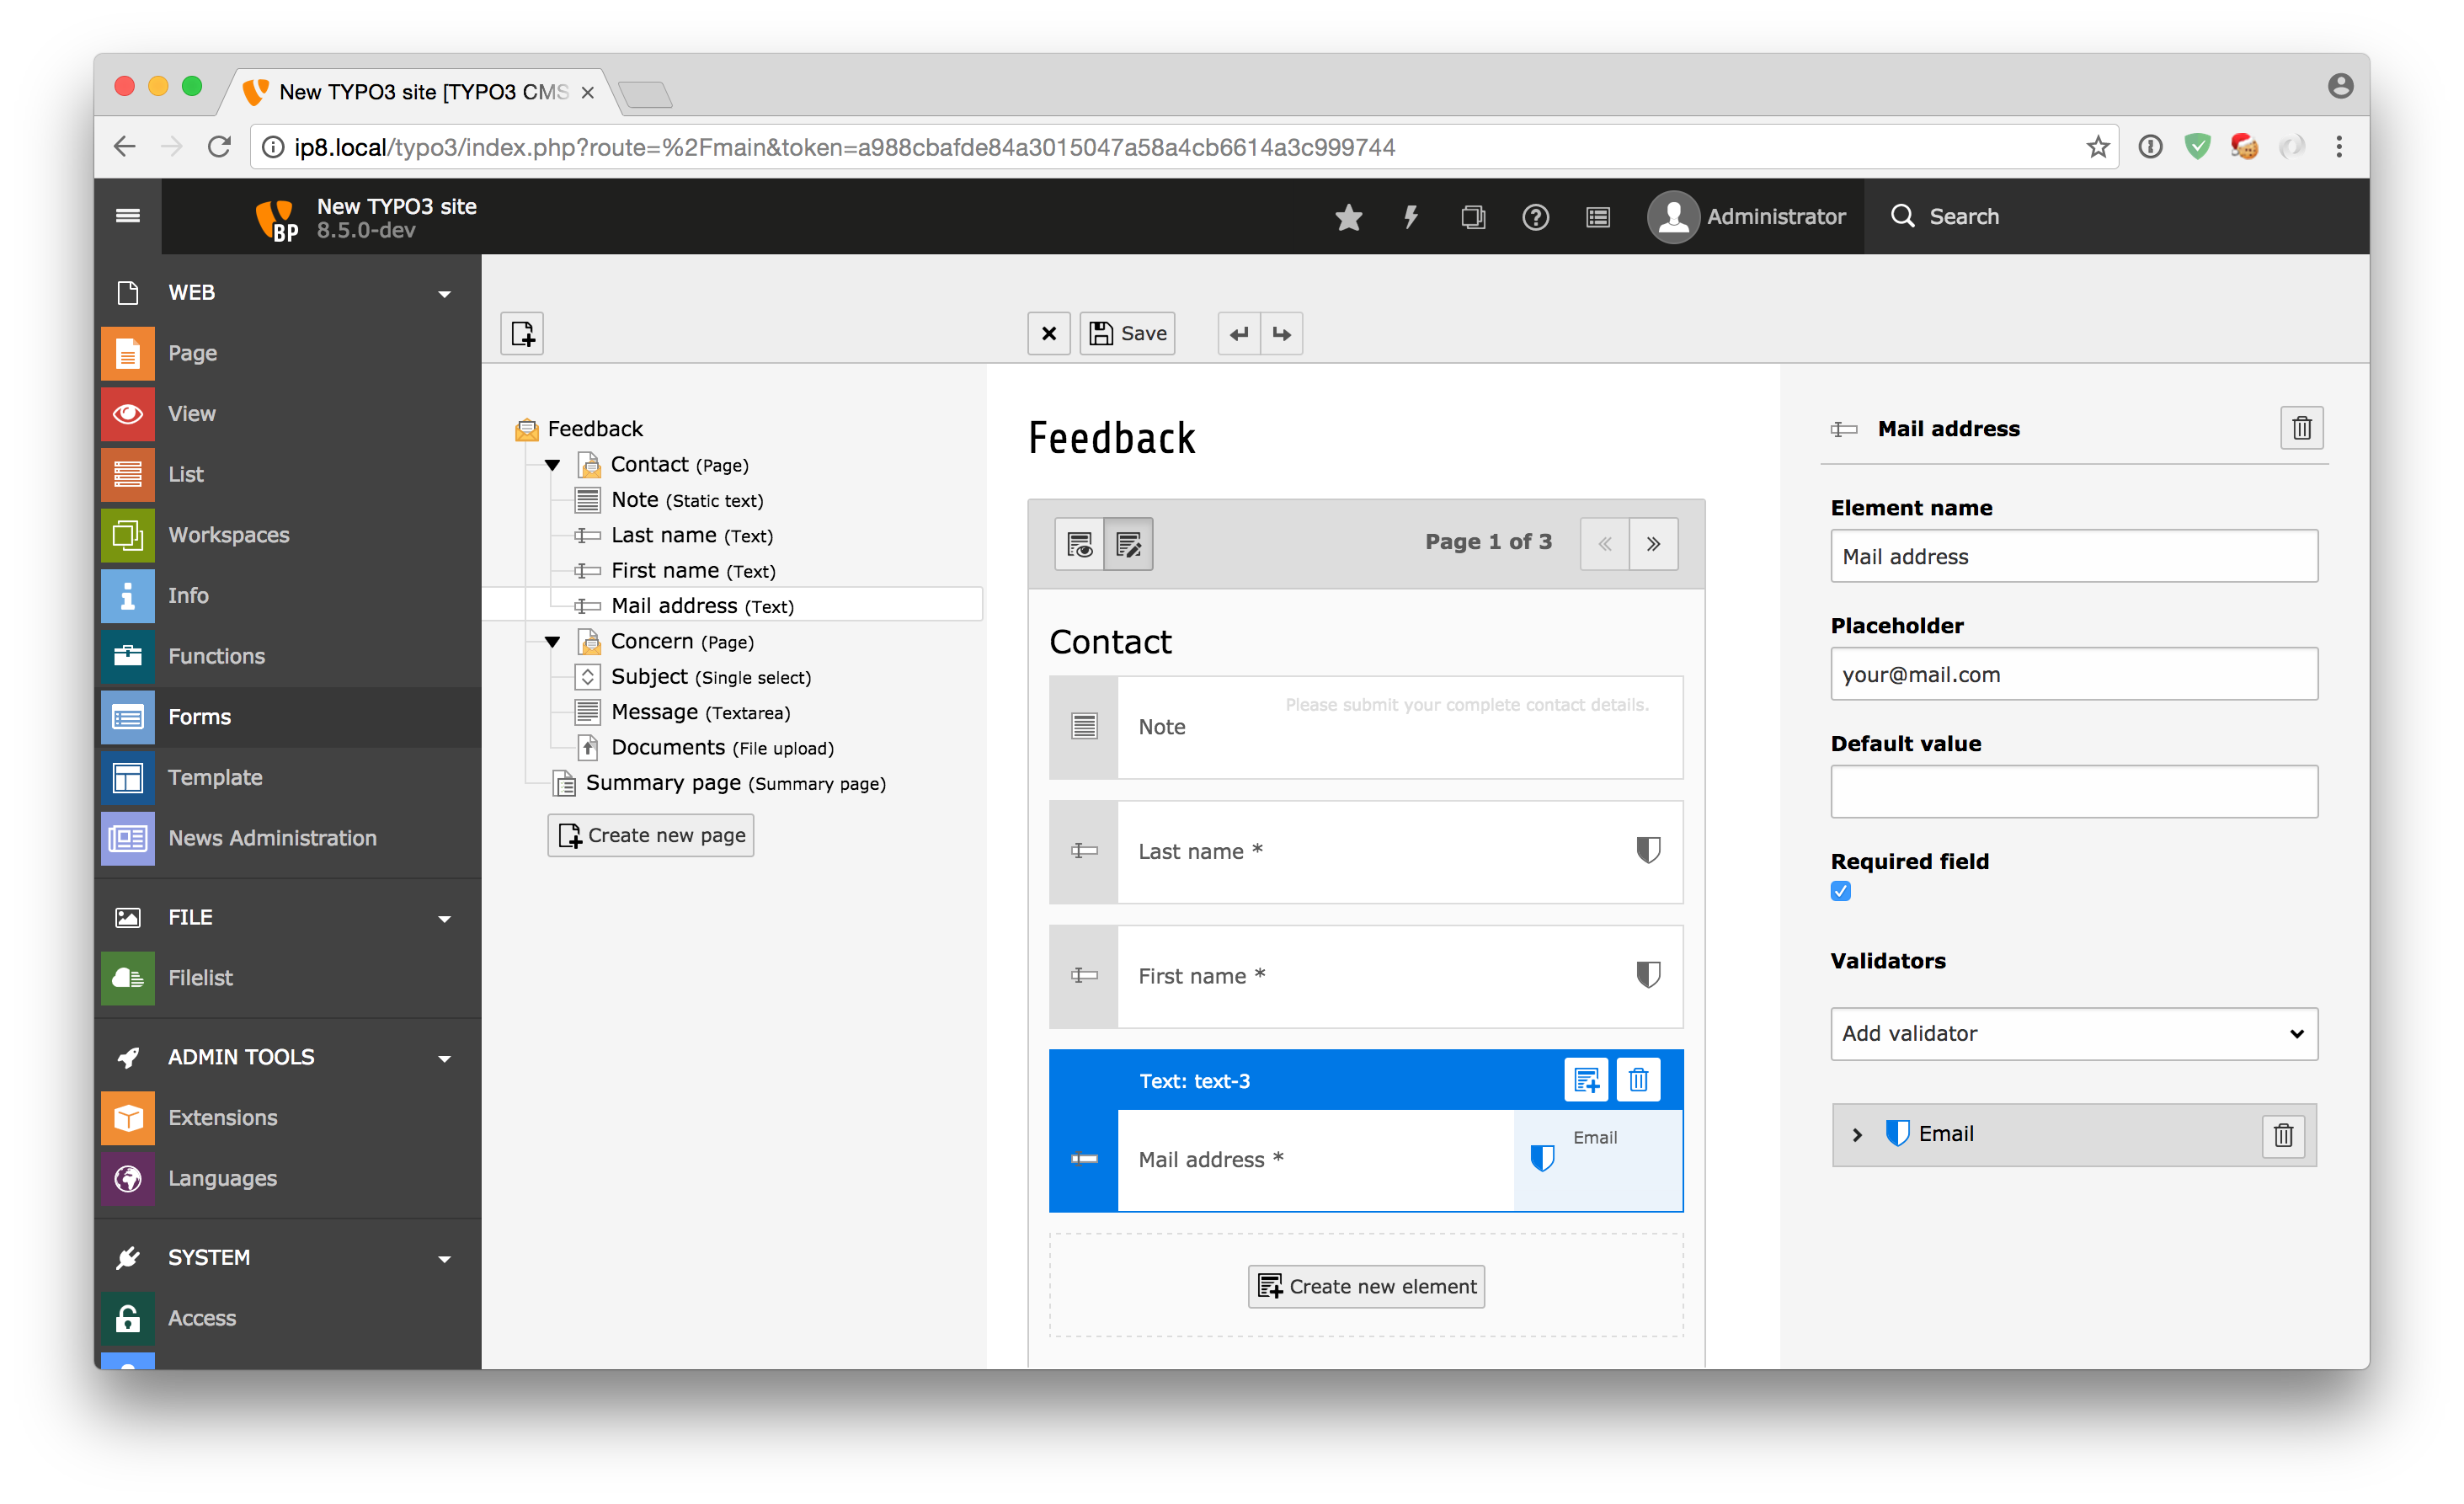
\includegraphics[width=0.8\linewidth]{BackendUserInterface/form-framework-1.png}
	\end{figure}

\end{frame}

% ------------------------------------------------------------------------------
% LTXE-SLIDE-START
% LTXE-SLIDE-UID:		1fc39608-885660d7-ee5ada39-82a54614
% LTXE-SLIDE-ORIGIN:	b91ec75b-7aa7b566-b523ca5f-f9ba3cde English
% LTXE-SLIDE-TITLE:		#77910: New Form Framework (3)
% ------------------------------------------------------------------------------
\begin{frame}[fragile]
	\frametitle{Interfaccia utente Backend}
	\framesubtitle{Nuovo Framework per i Form (3)}

	\begin{figure}
		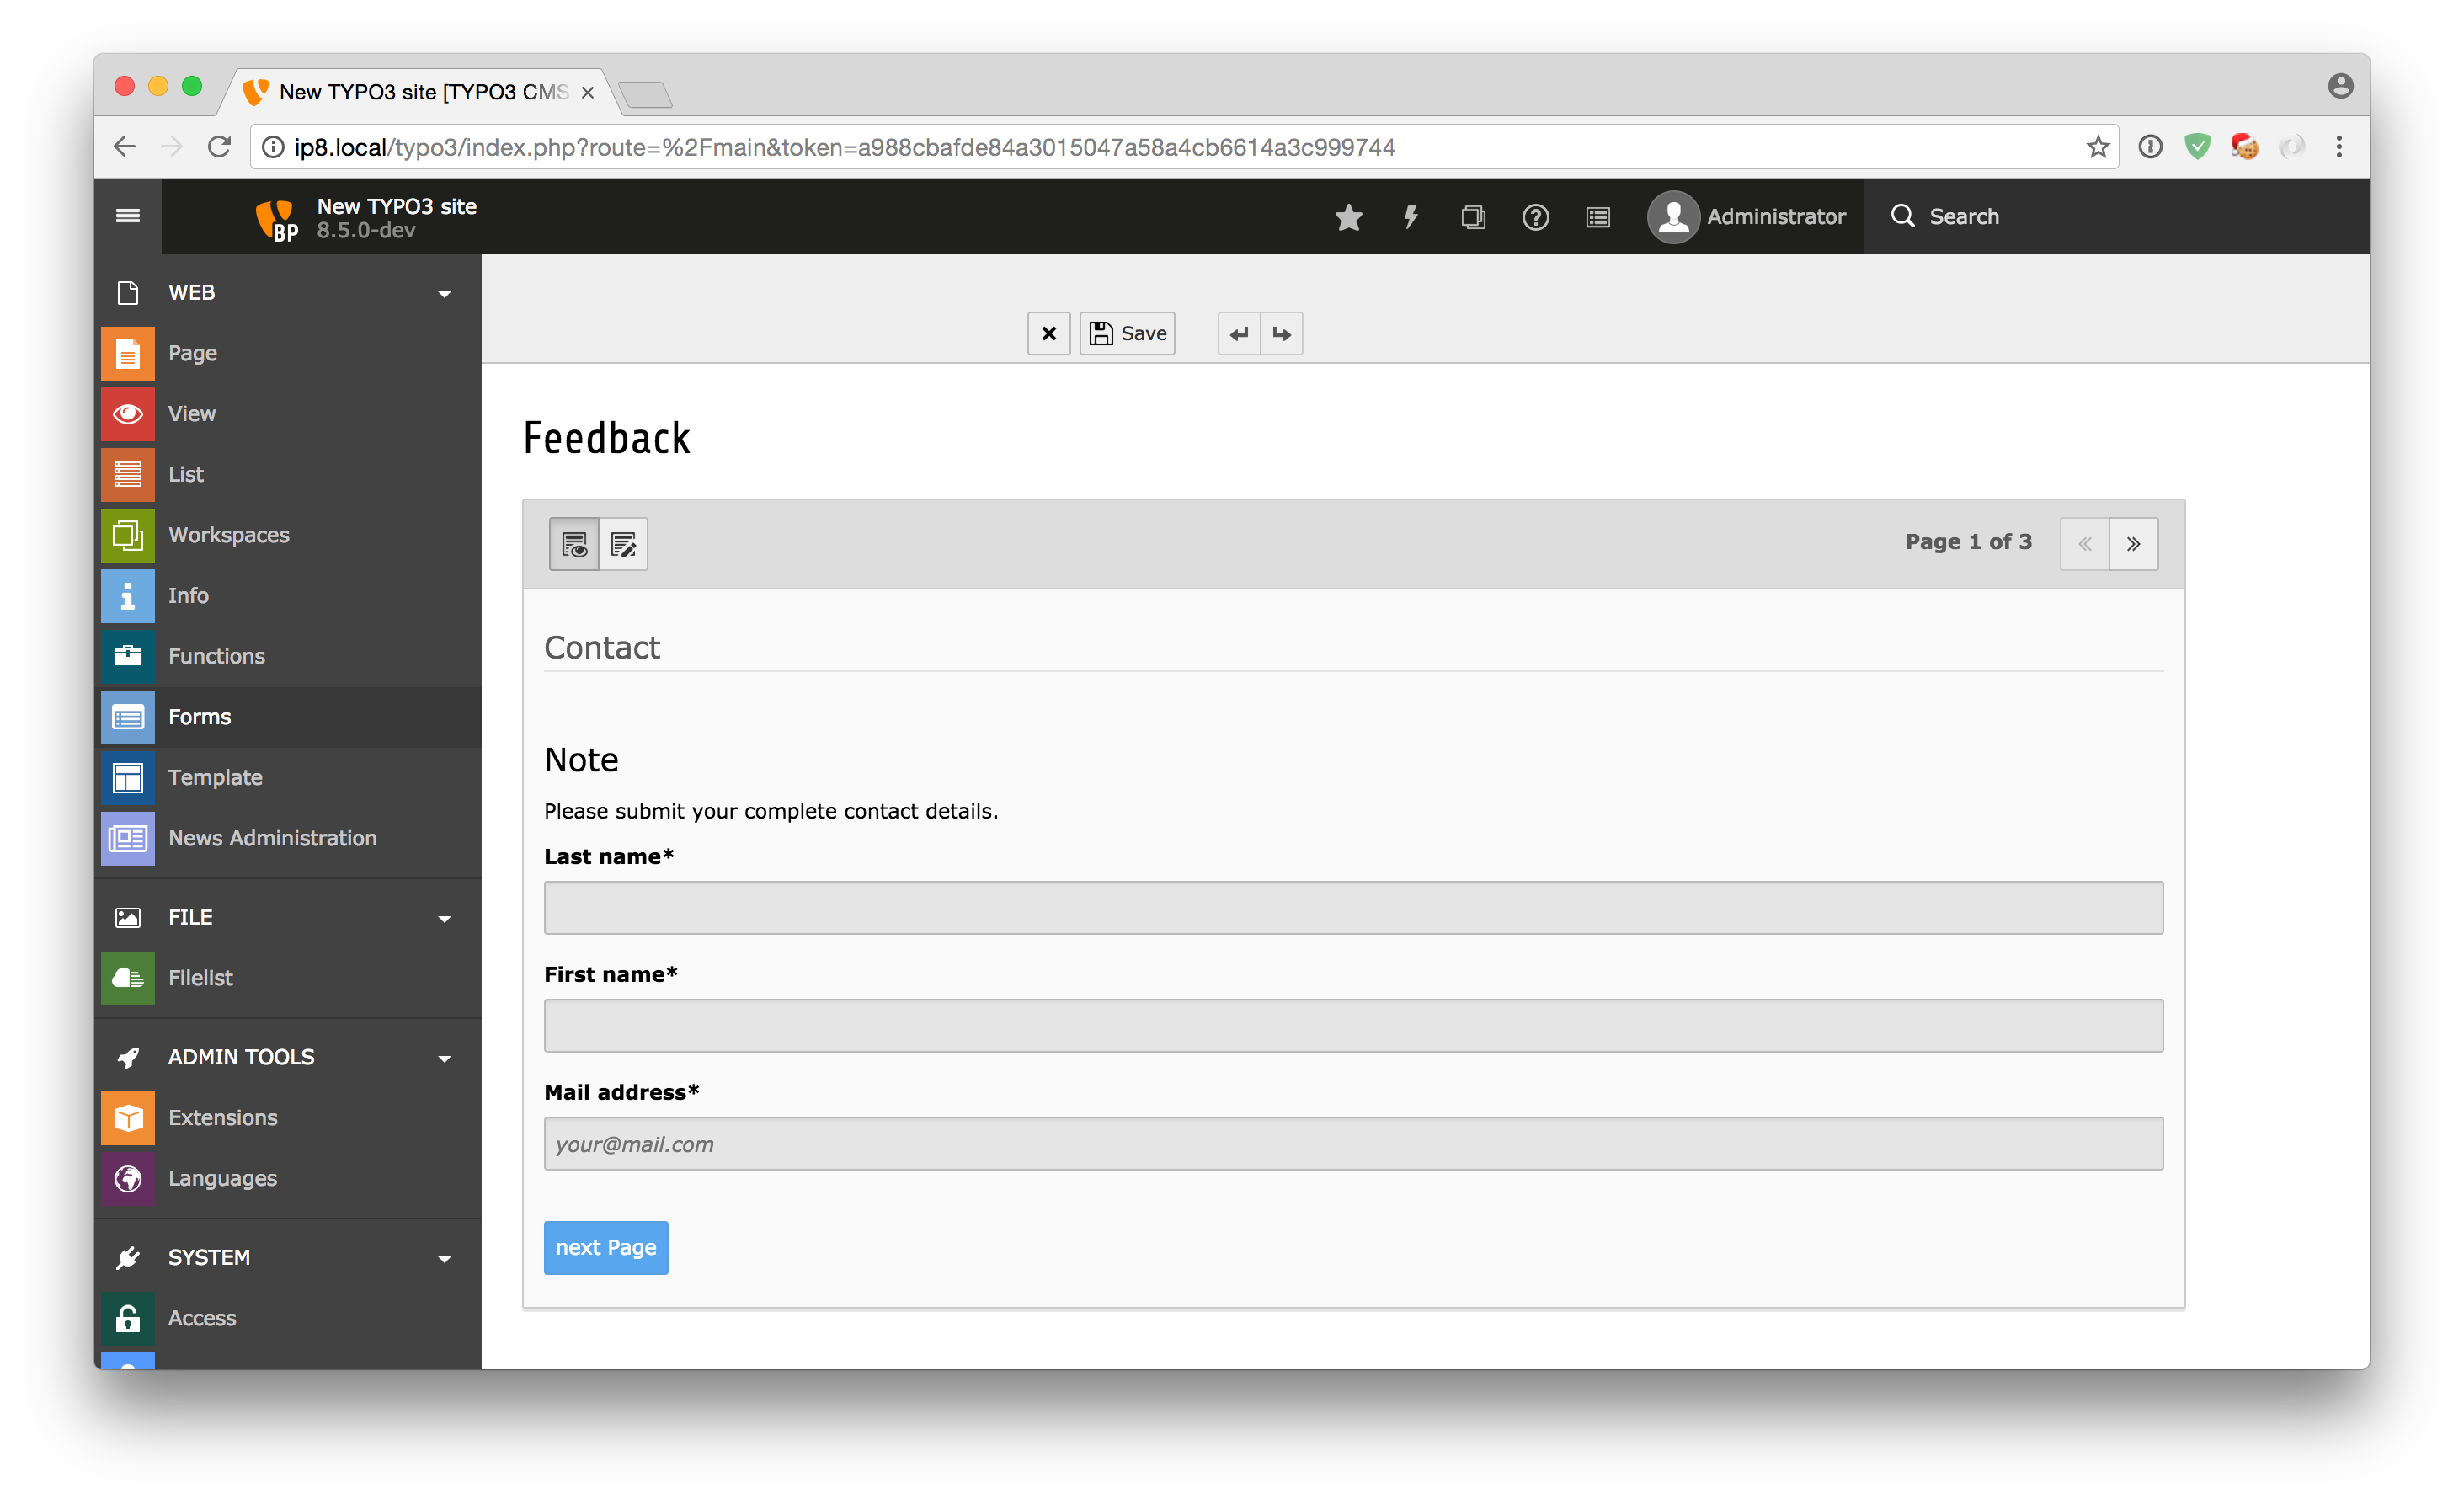
\includegraphics[width=0.8\linewidth]{BackendUserInterface/form-framework-2.png}
	\end{figure}

\end{frame}


% ------------------------------------------------------------------------------
% LTXE-SLIDE-START
% LTXE-SLIDE-UID:		8d5935d5-58da4379-f6053eda-19fe290e
% LTXE-SLIDE-ORIGIN:	c41b2f21-fb92bb80-56e7ddc9-1c725e34 English
% LTXE-SLIDE-TITLE:		CKEditor Integration
% ------------------------------------------------------------------------------
\begin{frame}[fragile]
	\frametitle{Interfaccia utente Backend}
	\framesubtitle{Integrazione CKEditor}

	\begin{columns}[T]
		\begin{column}{.5\textwidth}
			La nuova generazione dell'editing di testo è stata implementata nel backend di TYPO3:
			\textbf{CKEditor}.\newline

			L'attuale stato è volutamente marcato come \textit{experimental} e l'estensione 
			non è installata di default.\newline

			Maggiori dettagli su questo editor opensource: \url{http://ckeditor.com}
		\end{column}
		\begin{column}{.5\textwidth}
			\begin{figure}\vspace*{-0.4cm}
				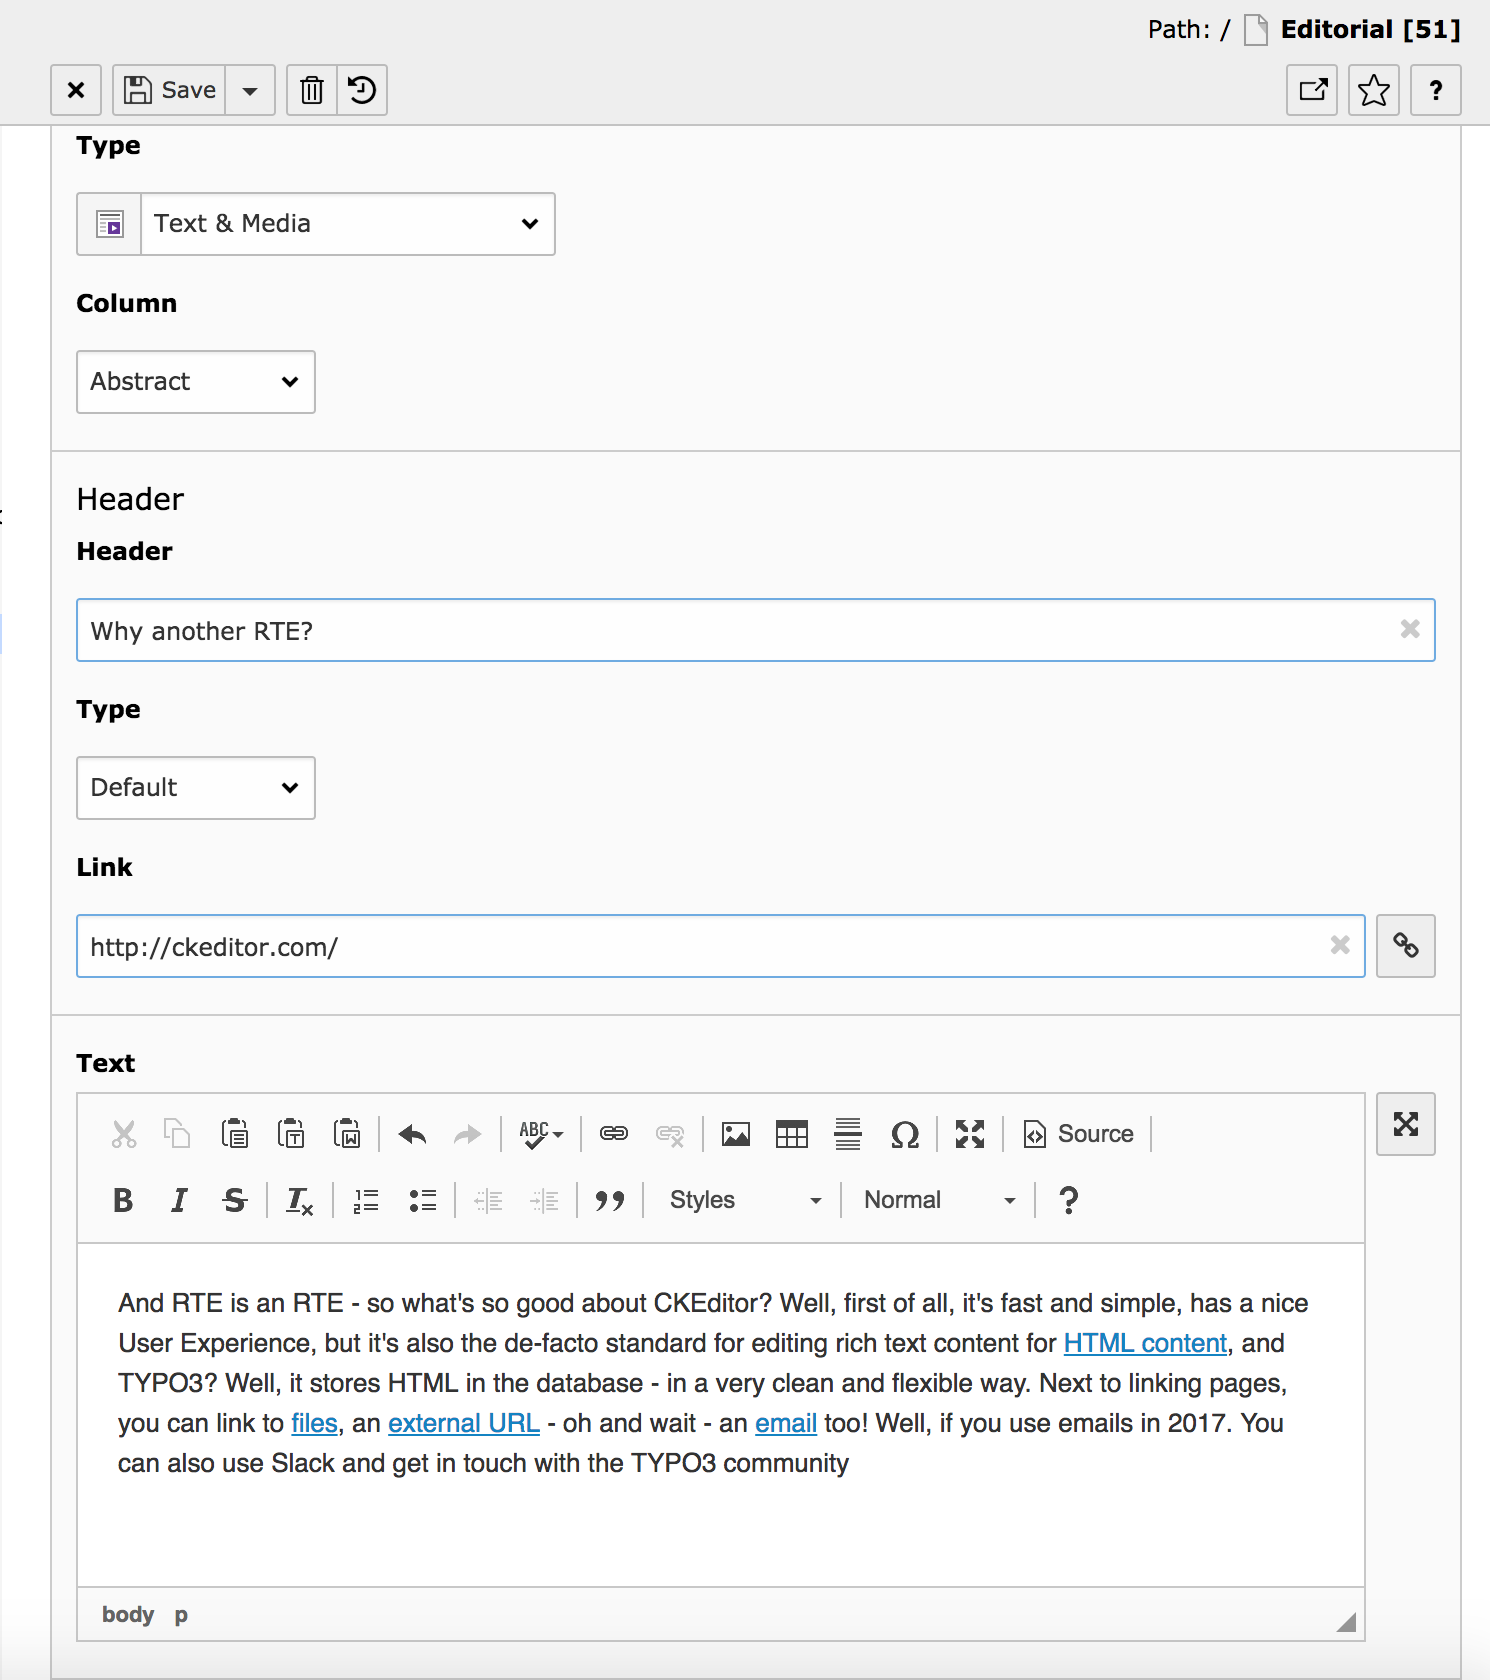
\includegraphics[width=0.8\linewidth]{BackendUserInterface/ckeditor.png}
			\end{figure}
		\end{column}
	\end{columns}

\end{frame}



% ------------------------------------------------------------------------------
% LTXE-SLIDE-START
% LTXE-SLIDE-UID:		dd593105-a2cca885-b8ed1841-d31e7d47
% LTXE-SLIDE-ORIGIN:	c9dc360d-cf218f95-03f53731-03d821ad English
% LTXE-SLIDE-TITLE:		#78383: Field positions in tabs streamlined (TCA)
% ------------------------------------------------------------------------------
\begin{frame}[fragile]
	\frametitle{Interfaccia utente Backend}
	\framesubtitle{Posizione e ordine degli elementi}

	\begin{itemize}
		\item L'ordine e la posizione di alcuni campi nel backend di TYPO3 è stato snellito
		\item L'obiettivo è quello di soddisfare le aspettative degli utenti su dove trovare opzioni dell'interfaccia utente usate di solito
		\item Questo è particolarmente importante per le definizioni ricorrenti dei campi e delle categorie generiche condivise da vari record
		\item Gli autori delle estensioni sono incoraggiati a seguire le posizioni e l'ordine degli elementi specificati
			nella \href{https://docs.typo3.org}{documentazione ufficiale}

			% TODO: update link above (waiting for Doc and Core Team to finish documentation)

	\end{itemize}

	\begin{itemize}
		\item \textit{La consistenza del backend è regina!} :-)
	\end{itemize}

\end{frame}

% ------------------------------------------------------------------------------
